This input does not follow a specific distribution but rather is a mix of the previous distributions.
The value is either chosen uniform random, from a binomial distribution, from a geometric distribution  or a powerlaw distribution.
One of the distributions is chosen uniform randomly.
This process is repeated $n$ times.
The values of this distribution then follow neither of the used distributions.

\begin{figure}[h]
      \caption{Distribution of a mixed input with \textasciitilde$U(1,999)$, \textasciitilde$B(1000,0.1)$, \textasciitilde$Geo(0.01)$, powerlaw dist with $\beta=-1.25$}
      \centering
      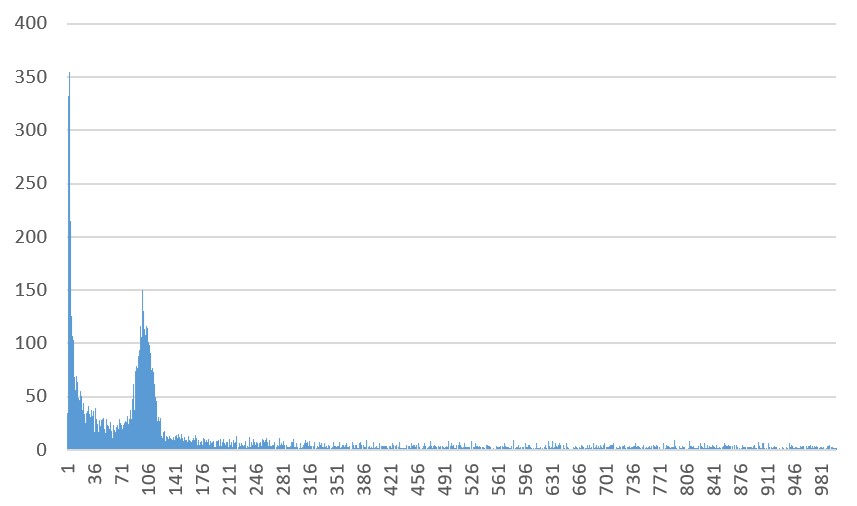
\includegraphics[width=0.7\textwidth]{figures/images/numberGenerator/mixed.png}\label{fig:mixedDistExample}
\end{figure}

The spike in the curve in Figure~\ref{fig:mixedDistExample} is caused by the binomial distribution with an expected value of 100.
Each value occurs at least 2.5 times in expectation due to the uniform distribution.
The large spike for the lowest values is caused by both the geometric and the powerlaw distribution.
The parameter for this figure were lowered to improve the visibility of bigger values which occurs much less frequently than the bigger values.
With a larger span of possible values the big values would be even less visible.

The used distributions for the experiments in the next subsections were \textasciitilde$U(1,49999)$, \textasciitilde$B(10000,0.1)$, \textasciitilde$Geo(0.001)$, powerlaw distribution with $\beta=-1.25$.